\documentclass[border=6pt]{standalone}
\usepackage{fontspec}
\setmainfont[
  Path = ../fonts/,
  UprightFont = Cabin-Regular.ttf,
  BoldFont = Cabin-Bold.ttf,
  ItalicFont = Cabin-Italic.ttf
]{Cabin}
\usepackage{amsmath, amssymb}
\usepackage{tikz}
\usetikzlibrary{arrows.meta, positioning, shapes.geometric}

\begin{document}
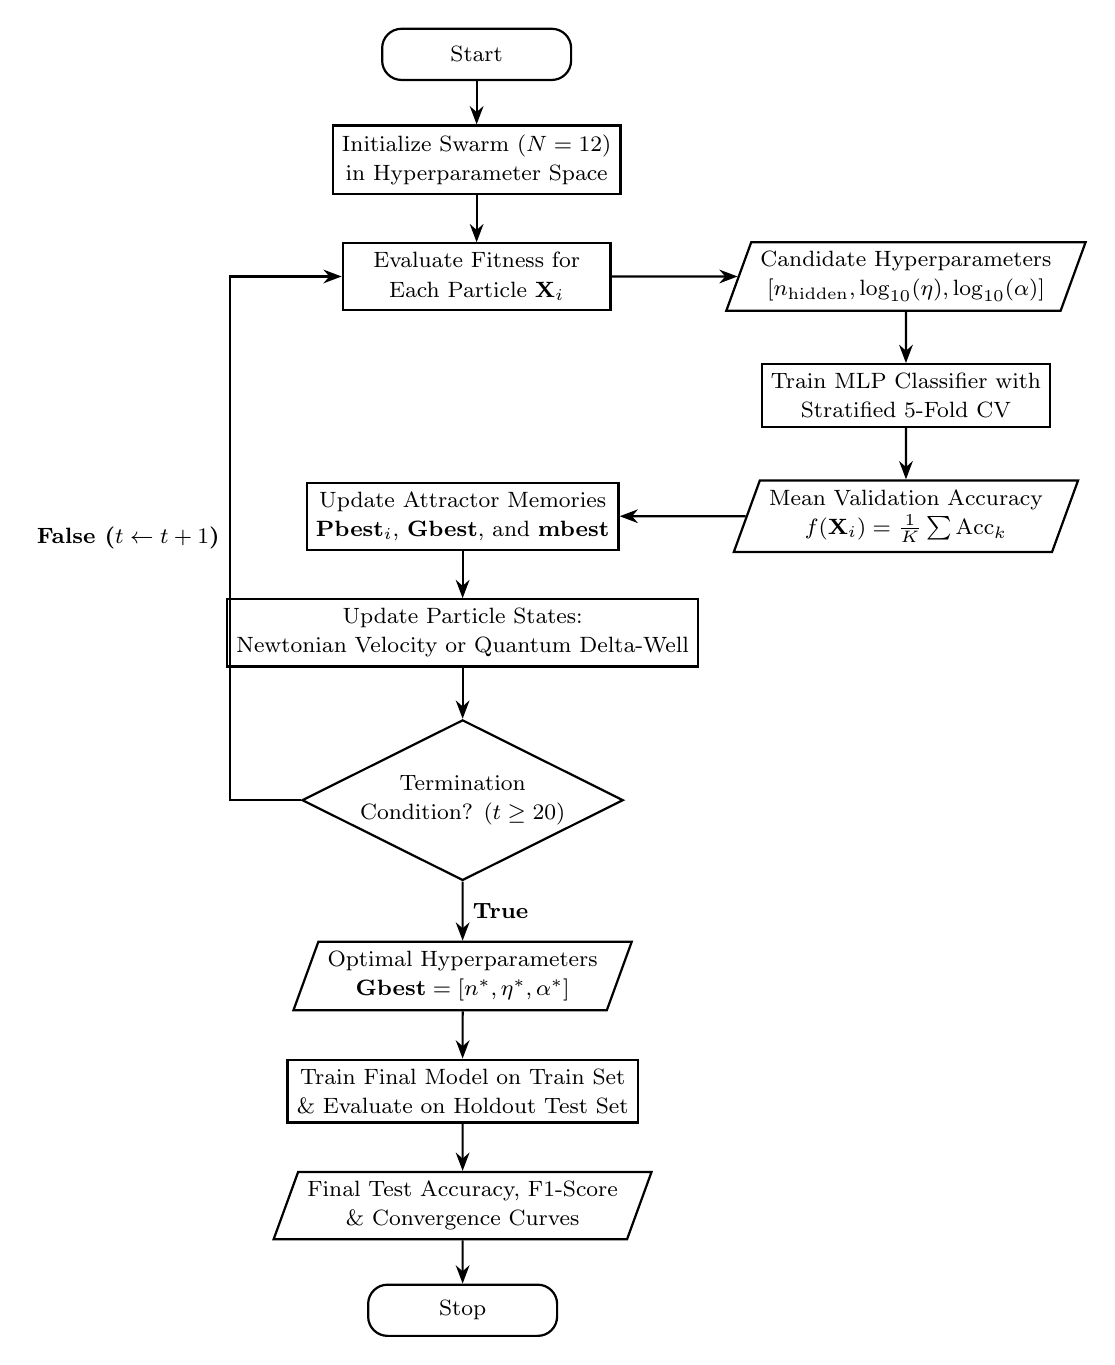
\begin{tikzpicture}[
    font=\fontsize{8.5pt}{10.5pt}\selectfont,
    >=Stealth,
    node distance=0.6cm and 1.8cm,
    startstop/.style={draw, rounded corners=7pt, minimum width=2.4cm, minimum height=0.65cm, align=center, line width=0.8pt},
    process/.style={draw, rectangle, minimum width=3.4cm, minimum height=0.75cm, align=center, line width=0.8pt},
    decision/.style={draw, diamond, aspect=2.0, minimum width=2.6cm, minimum height=0.85cm, align=center, line width=0.8pt, inner sep=1pt},
    data/.style={draw, trapezium, trapezium left angle=70, trapezium right angle=110, minimum width=3.0cm, minimum height=0.7cm, align=center, line width=0.8pt}
]

% Left Column: PSO Swarm Level
\node (start) [startstop] {Start};
\node (init) [process, below=0.55cm of start] {Initialize Swarm ($N=12$)\\in Hyperparameter Space};
\node (eval_swarm) [process, below=0.6cm of init] {Evaluate Fitness for\\Each Particle $\mathbf{X}_i$};

% Right Column: Neural Network Cross-Validation Evaluation
\node (params) [data, right=1.6cm of eval_swarm] {Candidate Hyperparameters\\$[n_{\mathrm{hidden}}, \log_{10}(\eta), \log_{10}(\alpha)]$};
\node (cv_train) [process, below=0.65cm of params] {Train MLP Classifier with\\Stratified 5-Fold CV};
\node (fitness_val) [data, below=0.65cm of cv_train] {Mean Validation Accuracy\\$f(\mathbf{X}_i) = \frac{1}{K}\sum \mathrm{Acc}_k$};

% Left Column Continuation: State Update & Convergence Check
\node (update_best) [process, left=1.6cm of fitness_val] {Update Attractor Memories\\$\mathbf{Pbest}_i$, $\mathbf{Gbest}$, and $\mathbf{mbest}$};
\node (update_particles) [process, below=0.6cm of update_best] {Update Particle States:\\Newtonian Velocity or Quantum Delta-Well};
\node (term) [decision, below=0.65cm of update_particles] {Termination\\Condition? ($t \ge 20$)};

% Bottom: Holdout Evaluation & Termination
\node (opt_params) [data, below=0.75cm of term] {Optimal Hyperparameters\\$\mathbf{Gbest} = [n^*, \eta^*, \alpha^*]$};
\node (test_eval) [process, below=0.6cm of opt_params] {Train Final Model on Train Set\\\& Evaluate on Holdout Test Set};
\node (final_results) [data, below=0.6cm of test_eval] {Final Test Accuracy, F1-Score\\\& Convergence Curves};
\node (stop) [startstop, below=0.55cm of final_results] {Stop};

% Arrows
\draw[->, line width=0.8pt] (start) -- (init);
\draw[->, line width=0.8pt] (init) -- (eval_swarm);

% Swarm to Evaluation
\draw[->, line width=0.8pt] (eval_swarm) -- (params);
\draw[->, line width=0.8pt] (params) -- (cv_train);
\draw[->, line width=0.8pt] (cv_train) -- (fitness_val);
\draw[->, line width=0.8pt] (fitness_val) -- (update_best);

% Update and Decision
\draw[->, line width=0.8pt] (update_best) -- (update_particles);
\draw[->, line width=0.8pt] (update_particles) -- (term);

% True condition
\draw[->, line width=0.8pt] (term) -- node[right, font=\footnotesize\bfseries] {True} (opt_params);
\draw[->, line width=0.8pt] (opt_params) -- (test_eval);
\draw[->, line width=0.8pt] (test_eval) -- (final_results);
\draw[->, line width=0.8pt] (final_results) -- (stop);

% False loop back
\draw[->, line width=0.8pt] (term.west) -- ++(-0.9,0) |- node[near start, left, font=\footnotesize\bfseries] {False ($t \leftarrow t+1$)} (eval_swarm.west);

\end{tikzpicture}
\end{document}
